\documentclass[11pt]{beamer}

\usepackage{array}    % <-- For defining new column types
\usepackage{booktabs}
\usepackage{hyperref}
\usepackage{makecell} % <-- For multi-line cells
\usepackage[default]{opensans} 
\usepackage{pgffor}
\usepackage{pdfpages}
\usepackage{palatino}  
\usepackage{tcolorbox} 
\usepackage{textcomp}
\usepackage{ulem}
\usepackage{xcolor} 
\usepackage{tcolorbox} 
\usepackage{tikz}
\usepackage{tabularx}



\usetikzlibrary{arrows.meta} 
\usetikzlibrary{decorations.pathreplacing} 
\usetikzlibrary{decorations.pathmorphing}  
\usetikzlibrary{decorations.markings}     
\usetikzlibrary{decorations.text}      

\usepackage{listings}
\lstset{
  basicstyle=\ttfamily\small,
  columns=fullflexible,
  breaklines=true,
  frame=single,
  showstringspaces=false,
  showspaces=false,
  keepspaces=true,
  tabsize=4
}


\newtcbox{\highlighttexttt}{nobeforeafter, colframe=white, colback=lightgray!30, boxrule=0pt, arc=2pt, boxsep=0pt, left=1pt, right=1pt, top=1pt, bottom=1pt}
\newcommand{\hl}[1]{\colorbox{lightgray!30}{\texttt{#1}}}
\newcommand{\blink}[2]{\href{#1}{\textcolor{blue}{\underline{#2}}}}
\newcommand{\try}[1]{Have A Try: \blink{https://github.com/FSU-COP4610-F25/in-class-code}{#1}}

\usetheme{Madrid}
\usefonttheme{default} 

\useinnertheme{circles}

\setbeamertemplate{footline}{
    \leavevmode%
    \hbox{%
        \begin{beamercolorbox}[wd=0.92\paperwidth,ht=2.5ex,dp=1ex,left]{section in head/foot}
            \hspace{0.5em}
            \insertsectionnavigationhorizontal{0.9\paperwidth}{}{}
        \end{beamercolorbox}%
        \begin{beamercolorbox}[wd=0.08\paperwidth,ht=2.5ex,dp=1ex,right]{section in head/foot}
            \insertframenumber{} / \inserttotalframenumber
            \hspace{0.2em}
        \end{beamercolorbox}%
    }%
    \vskip0pt%
}


\setbeamersize{text margin left=1em, text margin right=1em}

\setbeamertemplate{frametitle}{
    \vspace{-0.5em} 
    \begin{beamercolorbox}[wd=\paperwidth,ht=2.5ex,dp=0.75ex,left]{frametitle} 
        \usebeamerfont{frametitle}\hspace{0.72em}\insertframetitle
    \end{beamercolorbox}
    \vspace{-0.5em} 
}


\newcommand{\FSUOSMeta}{%
  \author[Xin Liu]{\small Xin Liu}%
  \institute[FSU]{\small Florida State University\\[2pt]
    \href{mailto:xliu15@fsu.edu}{xliu15@fsu.edu}}%
  \date[\today]{\small CIS 4930/5930 Future Edge Networks\\[2pt]
    {\footnotesize\href{https://xinliulab.github.io/FSU-CIS4930-CIS5930-Future-Edge-Networks/}
         {\mbox{xinliulab.github.io/FSU-CIS4930-CIS5930-Future-Edge-Networks}}}}%
}

%!TEX root = ./main.tex

% This deck uses \text{...} inside math and \gtrsim; the shared variables.tex does
% not load the AMS packages, so load them here.
\usepackage{amsmath,amssymb}

\usetikzlibrary{positioning,fit,backgrounds}
\usetikzlibrary{shapes.geometric,calc}

\definecolor{ranblue}{RGB}{46,91,186}
\definecolor{coreorange}{RGB}{222,122,36}
\definecolor{ranpurple}{RGB}{109,53,151}
\definecolor{softgreen}{RGB}{73,139,74}
\definecolor{softgray}{RGB}{92,98,105}

\newcommand{\source}[2]{%
  \par\vspace{0.25em}%
  {\tiny\textcolor{gray}{\href{#1}{\underline{#2}}}\par}%
}

% Inline expansion of an acronym at first use: SMS \expand{Short Message Service}
\newcommand{\expand}[1]{\textcolor{softgray}{(#1)}}

% Small gray glossary line, for slides with several acronyms at once.
\newcommand{\glossline}[1]{%
  \par\vspace{0.4em}%
  {\scriptsize\color{softgray}\raggedright#1\par}%
}

\newcommand{\plainterm}[2]{%
  \textbf{#1}\hspace{0.25em}{\small\textcolor{softgray}{#2}}%
}

\newcommand{\ask}[1]{%
  \begin{tcolorbox}[colback=blue!4,colframe=ranblue,boxrule=0.7pt,arc=2pt,
    left=5pt,right=5pt,top=4pt,bottom=4pt]
    \centering\large #1
  \end{tcolorbox}%
}

% Font is deliberately \normalsize, not \large: at \large a one-sentence takeaway
% wraps to two lines and the box grows into whatever is below it.
\newcommand{\takeaway}[1]{%
  \begin{tcolorbox}[colback=orange!7,colframe=coreorange,boxrule=0.7pt,arc=2pt,
    left=5pt,right=5pt,top=4pt,bottom=4pt]
    \centering\normalsize #1
  \end{tcolorbox}%
}

% Beamer overlays inside TikZ: \visible<...> breaks path parsing inside node text,
% so reveal nodes with the standard opacity idiom instead: \node[visible on=<2->] ...
\tikzset{
  invisible/.style={opacity=0,text opacity=0},
  visible on/.style={alt=#1{}{invisible}},
  alt/.code args={<#1>#2#3}{\alt<#1>{\pgfkeysalso{#2}}{\pgfkeysalso{#3}}},
}

\tikzset{
  netnode/.style={draw=ranblue,fill=blue!5,rounded corners=3pt,
    minimum width=1.9cm,minimum height=0.82cm,align=center,font=\bfseries},
  corenode/.style={draw=coreorange,fill=orange!7,rounded corners=3pt,
    minimum width=1.9cm,minimum height=0.82cm,align=center,font=\bfseries},
  oranode/.style={draw=ranpurple,fill=purple!6,rounded corners=3pt,
    minimum width=1.9cm,minimum height=0.82cm,align=center,font=\bfseries},
  flow/.style={-{Latex[length=2.4mm]},thick,draw=softgray}
}

% Full-width question/answer block: spans the whole frame, no box.
% Use below \end{columns} when the question is meant for the whole slide.
\newcommand{\qa}[2]{%
  \par\vspace{0.55em}%
  {\large\raggedright
    \noindent\hangindent=1.25em\hangafter=1
    \textcolor{ranblue}{\textbf{Q:}}\hspace{0.35em}\textbf{#1}\par
    \vspace{0.35em}
    \noindent\hangindent=1.25em\hangafter=1
    \textcolor{coreorange}{\textbf{A:}}\hspace{0.35em}#2\par}%
}

% ---------------------------------------------------------------------------
% Class 12 (Wi-Fi Sensing) additions.
% COLOR CONVENTION for this deck -- every figure obeys it:
%   ranblue    = the ANTENNA axis (space)      -> reading it gives angle
%   coreorange = the SUBCARRIER axis (frequency) -> reading it gives delay/distance
%   softgreen  = the direct path (the answer we want)
%   ranpurple  = reflected paths (multipath ghosts)
%   softgray   = hardware dirt: clocks, offsets, detection delay
%   talkred    = bad news (merged taps, broken assumptions)
% ---------------------------------------------------------------------------

\definecolor{talkred}{RGB}{163,26,52}

% One antenna element: a small triangle on a mast, pointing up. #1 = (x,y), #2 = color
\newcommand{\anttri}[2]{%
  \draw[#2,thick] ($#1+(-0.11,0.14)$) -- ($#1+(0,-0.06)$) -- ($#1+(0.11,0.14)$)
    -- cycle;
  \draw[#2,thick] ($#1+(0,-0.06)$) -- ($#1+(0,-0.22)$);%
}

% The CSI matrix: 3 antennas x 8 subcarriers, one phasor arrow per cell. The phase
% step per column (26 deg) and per row (90 deg = the running example's quarter turn)
% are EXAGGERATED on the frequency axis so students can see the twist; every frame
% that shows it says so in a gray caption. Draw inside a tikzpicture at the origin.
\newcommand{\csigrid}{%
  \foreach \m in {0,1,2}{
    \foreach \k in {0,...,7}{
      \draw[softgray!50,fill=gray!6] (\k*0.72,\m*0.72)
        rectangle ++(0.6,0.6);
      \pgfmathsetmacro{\ang}{100-26*\k-90*\m}
      \draw[-{Latex[length=1.3mm]},thick,black!70]
        (\k*0.72+0.3,\m*0.72+0.3) -- ++(\ang:0.21);
    }}
  % axis labels
  \draw[-{Latex[length=2mm]},thick,coreorange] (0,-0.42) -- (5.9,-0.42);
  \node[font=\scriptsize\bfseries,text=coreorange] at (2.95,-0.75)
    {subcarriers $f_1 \ldots f_K$ (frequency)};
  \draw[-{Latex[length=2mm]},thick,ranblue] (-0.42,0) -- (-0.42,2.2);
  \node[font=\scriptsize\bfseries,text=ranblue,rotate=90] at (-0.78,1.1)
    {antennas $1 \ldots M$};%
}


\title[Wi-Fi Sensing]{Class 12: Wi-Fi Sensing}
\subtitle{Angle from the Antennas, Distance from the Subcarriers}

\FSUOSMeta

\begin{document}

\begin{frame}[plain]
  \titlepage
\end{frame}

\addtocounter{framenumber}{-1}

% One straight line (2026-09-30). The whole lecture is one object -- the CSI matrix
% H[antenna, subcarrier] -- and one enemy -- phase wrapping. Each section defeats the
% enemy along one axis of the matrix, then SpotFi uses both axes at once.
% Sources this deck distills: the Tsinghua "Hands-on Wireless Sensing" tutorial (CSI
% model, ToF, AoA, MUSIC), the MIT localization lecture (RSSI-vs-phase hierarchy),
% ArrayTrack NSDI'13 (AoA), Chronos NSDI'16 (ToF), SpotFi SIGCOMM'15 (joint 2D).
%!TEX root = ./main.tex

\section[The idea]{The Idea: Phase Is a Ruler}

% SECTION TIMING: 0:00--8:00 (2 frames).
% LAYOUT RULES for this template:
%   - a frame title must fit ONE line in the title bar: keep it under ~44 characters.
%   - every bullet must fit on one line; shorten the text, do not let it wrap.
% RUNNING EXAMPLE for the whole deck -- keep the numbers consistent everywhere:
%   5 GHz Wi-Fi, wavelength 6 cm, antenna spacing d = 3 cm (half wavelength).
%   Direct path: phone at 30 degrees, 5 m  (delay ~17 ns).
%   Wall echo:   arrives from -40 degrees, 8 m path (delay ~27 ns).
%   At 30 degrees, each next antenna lags by pi/2 -- a QUARTER TURN. Say it that way.

% Teaching note (240 s): read the three cards slowly; each is a real, published
% result, not a demo video. Then ask the Q out loud and let the room guess sensors
% (camera? UWB? radar chip?) before revealing that the answer is "none".
\begin{frame}{What your access point knows without asking}
  \vspace{0.5em}
  \centering
  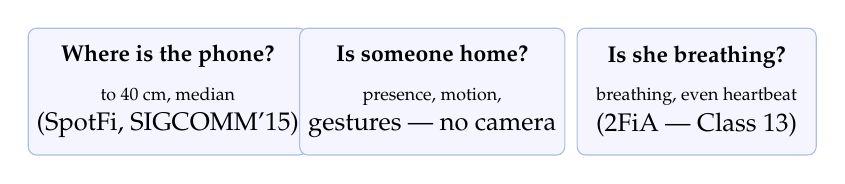
\begin{tikzpicture}[scale=0.92,transform shape]
    \foreach \i/\head/\body in {
      0/{Where is the phone?}/{to 40 cm, median\\(SpotFi, SIGCOMM'15)},
      1/{Is someone home?}/{presence, motion,\\gestures --- no camera},
      2/{Is she breathing?}/{breathing, even heartbeat\\(2FiA --- Class 13)}}{
      \node[draw=ranblue!40,fill=blue!4,rounded corners=3pt,minimum width=3.3cm,
            minimum height=1.75cm,align=center] at (\i*3.65,0)
        {\small\textbf{\head}\\[3pt]\scriptsize\body};
    }
  \end{tikzpicture}

  \vspace{0.3em}
  \qa{Which extra sensor did the access point need for all of this?}
     {None. Every answer was read out of the \textbf{channel estimates} the AP
      already computes just to decode packets. This lecture is about how.}

  \source{https://dl.acm.org/doi/10.1145/2785956.2787487}{Kotaru et al., SpotFi, SIGCOMM 2015 \quad$\cdot$\quad 2FiA appears in Paper Practicum 5 (Class 13)}
\end{frame}

% Teaching note (240 s): the one contrast the section exists for. RSSI collapses the
% whole room into one number; phase turns 360 degrees every 6 cm of path. Do the
% mental arithmetic on the slide out loud: 1 degree ~ 0.17 mm. Then the honest catch:
% that exquisite ruler has no absolute markings -- which is the next frame's problem.
\begin{frame}{RSSI is a light meter, phase is a ruler}
  \vspace{0.4em}
  \begin{columns}[T,onlytextwidth]
    \column{0.47\textwidth}
      {\small\textbf{\textcolor{softgray}{RSSI --- signal strength}}\par}
      \vspace{0.4em}
      {\small
       \begin{itemize}\itemsep4pt
         \item One number per packet.
         \item All paths, summed as power.
         \item Swings dBs if you just stand up.
         \item Good for: rough presence.
       \end{itemize}\par}
    \column{0.47\textwidth}
      {\small\textbf{\textcolor{ranblue}{Phase --- of the channel $H$}}\par}
      \vspace{0.4em}
      {\small
       \begin{itemize}\itemsep4pt
         \item One per subcarrier, per antenna.
         \item Turns $360^\circ$ every wavelength.
         \item At 5 GHz: $\lambda = 6$ cm.
         \item $1^\circ$ of phase $\approx$ 0.17 mm of path.
       \end{itemize}\par}
  \end{columns}

  \vspace{0.8em}
  \takeaway{Wi-Fi sensing is the move from reading \textcolor{softgray}{power}\\
    to reading \textcolor{ranblue}{phase} --- from a light meter to a ruler.}

  \source{https://www.mit.edu/~fadel/courses/MAS.s60/materials/Lec2-localization-2022.pdf}{Adib, MIT MAS.S60, Lecture 2: RF localization --- the RSSI-to-phase hierarchy}
\end{frame}
      % what a stock AP has sensed; RSSI is a light meter
%!TEX root = ./main.tex

\section[CSI]{CSI: The Measurement You Already Have}

% SECTION TIMING: 8:00--22:00 (4 frames).
% Job of the section: put ONE object on the table -- the matrix H[antenna,
% subcarrier] -- and ONE enemy -- wrapping. Everything after is reading that
% matrix along one axis or the other. Students met subcarriers and training
% fields in Class 8; lean on that, do not re-teach OFDM.

% Teaching note (210 s): start from decoding, not from sensing. Ask: the wave
% arrives scaled and rotated -- how does the receiver know what "1+0j" was supposed
% to look like? Answer: the preamble. H falls out as a by-product on every packet.
\begin{frame}{The receiver must learn H before bit one}
  \vspace{0.3em}
  {\small Every packet opens with training symbols the receiver already knows
   (Class 8).\par}
  \vspace{0.3em}
  {\small On each subcarrier $f$ and each antenna, the receiver solves\par}
  \vspace{0.2em}
  \centering
  {\large $y = H \cdot x_{\text{known}} \;\;\Rightarrow\;\;
    H = y / x_{\text{known}}$\par}
  \vspace{0.6em}
  \raggedright
  {\small $H$ is one \textbf{complex number}: $|H|$ says how much the wave faded,
   $\arg H$ says\par}
  {\small how far it travelled --- for a single path of length $r$:\par}
  \vspace{0.2em}
  \centering
  {\large $H = \alpha\, e^{-j 2\pi f\, r/c}$
   \quad{\small\textcolor{softgray}{(one turn of phase per wavelength of $r$)}}\par}

  \vspace{0.7em}
  \qa{What does the modem do with $H$ after equalizing the packet?}
     {Throws it away --- thousands of times per second. CSI tools simply
      \emph{keep} it. Sensing is recycling.}

  \glossline{CSI = Channel State Information: the collection of these $H$ values
    \quad $c$ = speed of light}
\end{frame}

% Teaching note (180 s): the star figure of the lecture -- it returns in the SpotFi
% section with arrows on it. Point at one cell: one complex number. Then sweep a row,
% then a column. Do NOT yet say what the twists mean; just make them see the grid.
\begin{frame}{Ninety numbers per packet, for free}
  \vspace{0.3em}
  \centering
  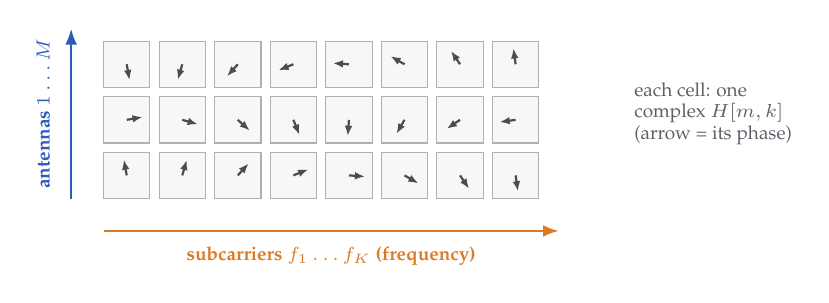
\begin{tikzpicture}[scale=0.98,transform shape]
    \csigrid
    \node[font=\scriptsize,align=left,text=softgray] at (7.9,1.1)
      {each cell: one\\complex $H[m,k]$\\(arrow = its phase)};
  \end{tikzpicture}

  \vspace{0.5em}
  \raggedright
  {\small
   \begin{itemize}\itemsep3pt
     \item The classic Intel 5300 tool exports $3$ antennas $\times$ $30$
       subcarriers $=$ \textbf{90 complex values per packet}.
     \item Hundreds of packets per second $\Rightarrow$ a \emph{movie} of the
       channel: $H[\text{time},\, \text{antenna},\, \text{subcarrier}]$.
   \end{itemize}\par}

  {\scriptsize\color{softgray}Phase twists exaggerated on the frequency axis so
   they are visible.\par}

  \source{https://dhalperi.github.io/linux-80211n-csitool/}{Halperin et al., Linux 802.11n CSI Tool \quad$\cdot$\quad Tsinghua Wireless Sensing Tutorial, ``Understanding CSI''}
\end{frame}

% Teaching note (210 s): introduce the running example here and never change it:
% direct path 5 m at +30 deg (green), wall echo 8 m at -40 deg (purple). The formula
% is shown ONCE, then immediately translated into the three per-path words.
\begin{frame}{The room writes itself into the matrix}
  \vspace{0.2em}
  \centering
  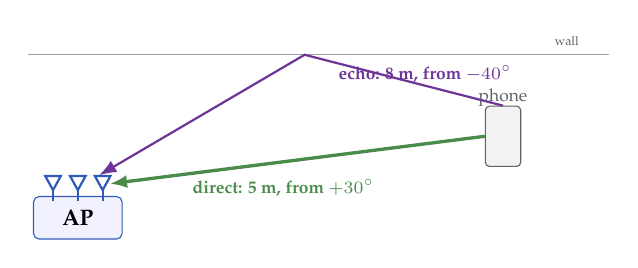
\begin{tikzpicture}[scale=0.9,transform shape]
    % the room
    \draw[softgray!60] (0,2.6) -- (8.2,2.6);
    \node[font=\tiny,text=softgray] at (7.6,2.8) {wall};
    % AP with 3 antennas
    \node[draw=ranblue,fill=blue!5,rounded corners=2pt,minimum width=1.25cm,
          minimum height=0.6cm,font=\bfseries\small] (ap) at (0.7,0.3) {AP};
    \anttri{(0.35,0.75)}{ranblue}
    \anttri{(0.70,0.75)}{ranblue}
    \anttri{(1.05,0.75)}{ranblue}
    % phone
    \node[draw=softgray,fill=gray!10,rounded corners=1.5pt,minimum width=0.5cm,
          minimum height=0.85cm,font=\scriptsize] (ph) at (6.7,1.45) {\phantom{.}};
    \node[font=\scriptsize,text=softgray] at (6.7,2.0) {phone};
    % direct path
    \draw[-{Latex[length=2.2mm]},very thick,softgreen] (ph.west) -- (1.15,0.78);
    \node[font=\scriptsize\bfseries,text=softgreen] at (3.6,0.72)
      {direct: 5 m, from $+30^\circ$};
    % wall echo
    \draw[-{Latex[length=2.2mm]},thick,ranpurple] (ph.north) -- (3.9,2.6)
      -- (1.0,0.9);
    \node[font=\scriptsize\bfseries,text=ranpurple] at (5.6,2.33)
      {echo: 8 m, from $-40^\circ$};
  \end{tikzpicture}

  \vspace{0.4em}
  {\small Each path $\ell$ stamps the whole matrix at once:\par}
  \vspace{0.15em}
  \centering
  {\normalsize $H[m,k] \;=\; \sum_{\ell}\; \alpha_\ell\;
    \underbrace{e^{-j 2\pi f_k \tau_\ell}}_{\textcolor{coreorange}{\text{delay
    } \tau_\ell}}\;
    \underbrace{e^{-j \frac{2\pi}{\lambda} m d \sin\theta_\ell}}_{%
    \textcolor{ranblue}{\text{angle } \theta_\ell}}$\par}

  \vspace{0.45em}
  \takeaway{The AP receives only the \textbf{sum}. Sensing is un-summing:\\
    recover each path's $(\theta_\ell, \tau_\ell)$ from the matrix.}
\end{frame}

% Teaching note (180 s): the enemy, named once, properly. The odometer picture does
% the work: you see the dial, not the mileage. Close with the roadmap takeaway and
% point at the two colored axes -- that IS the table of contents of the lecture.
\begin{frame}{The catch: every phase arrives wrapped}
  \vspace{0.3em}
  \begin{columns}[T,onlytextwidth]
    \column{0.36\textwidth}
      \centering
      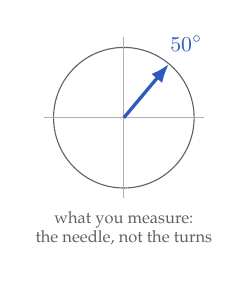
\begin{tikzpicture}[scale=0.85,transform shape]
        \draw[softgray] (0,0) circle (1.05);
        \draw[softgray!50] (-1.2,0) -- (1.2,0);
        \draw[softgray!50] (0,-1.2) -- (0,1.2);
        \draw[-{Latex[length=2.4mm]},very thick,ranblue] (0,0) -- (50:1.05);
        \node[font=\small\bfseries,text=ranblue] at (50:1.45) {$50^\circ$};
        \node[font=\scriptsize,text=softgray,align=center] at (0,-1.65)
          {what you measure:\\the needle, not the turns};
      \end{tikzpicture}
    \column{0.60\textwidth}
      {\small Our 5 m direct path at $f = 5.2$ GHz has turned\par}
      \vspace{0.15em}
      {\small \centering $f \cdot \tau \;\approx\; 5.2\,\text{GHz} \times 17\,
        \text{ns} \;\approx\; \text{\textbf{87 full turns}}$.\par}
      \vspace{0.4em}
      {\small The receiver sees only the leftover fraction ---
       like an odometer showing nothing but its last digit.\par}
      \vspace{0.4em}
      {\small One phase reading says: ``the path is $x + n\cdot 6$ cm,
       for \emph{some} integer $n$.'' Useless alone.\par}
  \end{columns}

  \vspace{0.6em}
  \takeaway{The fix is never one reading --- it is a \textbf{difference} along
    an axis:\\across \textcolor{ranblue}{antennas} $\to$ \textbf{angle};\;
    across \textcolor{coreorange}{subcarriers} $\to$ \textbf{distance}.}
\end{frame}
       % the matrix you already have, and why phase wraps
%!TEX root = ./main.tex

\section[Angle]{Ruler 1: Angle, Read Across the Antennas}

% SECTION TIMING: 22:00--40:00 (6 frames). This is ArrayTrack's story, told on the
% running example. The section's one sentence: the SAME wavefront hits each antenna
% at a slightly different time, so the phase STEP between neighbors encodes the
% direction -- and a step is a difference, so wrapping is beaten.

% Teaching note (150 s): pure intuition, zero math. Snap your fingers on the left of
% the room: which ear heard it first? The brain does AoA from micro-delays; the AP
% does it from phase. Only then advance to the geometry.
\begin{frame}{Two ears, one voice}
  \vspace{0.3em}
  \centering
  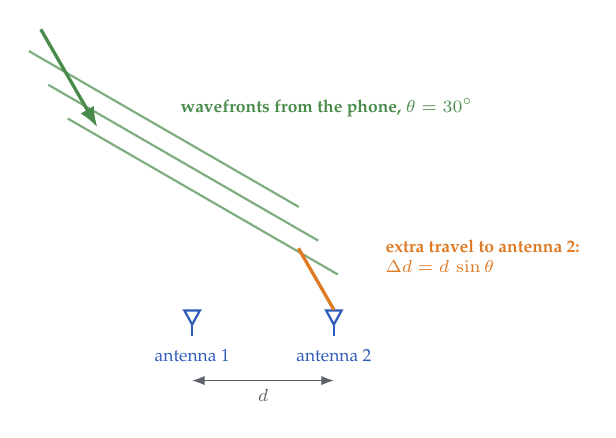
\begin{tikzpicture}[scale=0.9,transform shape]
    % incoming plane wavefronts at 30 degrees from boresight (i.e. tilted)
    \foreach \s in {0,0.55,1.1}{
      \draw[softgreen!70,thick] ($(1.1,3.3)+(-60:\s)+(150:2.2)$)
        -- ($(1.1,3.3)+(-60:\s)-(150:2.2)$);}
    \draw[-{Latex[length=2.6mm]},very thick,softgreen]
      (1.1,3.3) ++(150:1.6) ++(-60:-0.7) -- ++(-60:1.6);
    \node[font=\scriptsize\bfseries,text=softgreen] at (3.4,3.6)
      {wavefronts from the phone, $\theta = 30^\circ$};
    % two antennas
    \anttri{(1.5,0.6)}{ranblue}
    \anttri{(3.5,0.6)}{ranblue}
    \node[font=\scriptsize,text=ranblue] at (1.5,0.1) {antenna 1};
    \node[font=\scriptsize,text=ranblue] at (3.5,0.1) {antenna 2};
    \draw[softgray,{Latex[length=1.6mm]}-{Latex[length=1.6mm]}]
      (1.5,-0.25) -- node[below,font=\scriptsize]{$d$} (3.5,-0.25);
    % extra path to antenna 2
    \draw[very thick,coreorange] (3.5,0.75) -- ++(120:1.0);
    \node[font=\scriptsize\bfseries,text=coreorange,align=left] at (5.6,1.5)
      {extra travel to antenna 2:\\$\Delta d = d\,\sin\theta$};
  \end{tikzpicture}

  \vspace{0.5em}
  \qa{The wavefront is a straight line. Why does antenna 2 hear it late?}
     {Because the line is \emph{tilted} by the arrival angle $\theta$. The lag
      \textbf{is} the direction --- your ears run this algorithm all day.}
\end{frame}

% Teaching note (210 s): the worked number is the point of the frame. d = 3 cm,
% lambda = 6 cm, theta = 30 deg: a quarter turn per antenna. Have them compute the
% step for theta = 0 (zero) and theta = 90 (half turn) -- the full dial.
\begin{frame}{The phase difference is the angle}
  \vspace{0.4em}
  \centering
  {\large $\Delta\varphi \;=\; \dfrac{2\pi}{\lambda}\, d \sin\theta$\par}
  \vspace{0.35em}
  {\small\textcolor{softgray}{extra path $d\sin\theta$, charged at one turn per
    wavelength}\par}

  \vspace{0.6em}
  \begin{tcolorbox}[colback=green!5,colframe=softgreen,boxrule=0.7pt,arc=2pt,
    left=5pt,right=5pt,top=4pt,bottom=4pt,width=0.9\textwidth]
    \small\centering
    Running example: $\lambda = 6$ cm, $d = 3$ cm, phone at $\theta = 30^\circ$
    \\[3pt]
    $\Delta\varphi = \frac{2\pi}{6\,\text{cm}} \cdot 3\,\text{cm} \cdot
     \sin 30^\circ = \pi/2$ \;---\; \textbf{a quarter turn per antenna}
  \end{tcolorbox}

  \vspace{0.5em}
  \qa{Why do arrays space antennas exactly $d = \lambda/2$?}
     {Wrapping, again. At $d = \lambda/2$, $\Delta\varphi = \pi\sin\theta$ stays
      inside $(-\pi, \pi]$: every angle gets its \emph{own} phase step. Space
      them wider and two directions share one reading.}
\end{frame}

% Teaching note (180 s): from one step to a pattern. Three antennas at 30 deg read
% 0, 90, 180 degrees -- a straight line in antenna index. Name "steering vector" as
% nothing more than "the pattern angle theta WOULD produce".
\begin{frame}{M antennas: the phases form a line}
  \vspace{0.3em}
  \centering
  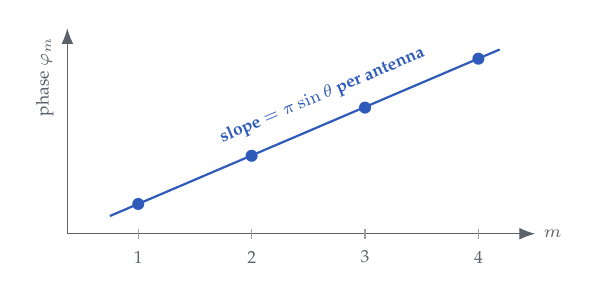
\begin{tikzpicture}[scale=0.9,transform shape]
    % axes
    \draw[-{Latex[length=2mm]},softgray] (0,0) -- (6.6,0)
      node[right,font=\scriptsize]{$m$};
    \draw[-{Latex[length=2mm]},softgray] (0,0) -- (0,2.9)
      node[rotate=90,font=\scriptsize,anchor=south east,yshift=2pt]{phase $\varphi_m$};
    \foreach \m/\x in {1/1.0, 2/2.6, 3/4.2, 4/5.8}{
      \draw[softgray!60] (\x,-0.07) -- (\x,0.07);
      \node[font=\scriptsize,text=softgray] at (\x,-0.33) {\m};}
    % the line through measured points
    \draw[ranblue,thick] (0.6,0.25) -- (6.1,2.6);
    \foreach \x/\y in {1.0/0.42, 2.6/1.10, 4.2/1.78, 5.8/2.47}{
      \fill[ranblue] (\x,\y) circle (0.085);}
    \node[font=\scriptsize\bfseries,text=ranblue,rotate=23] at (3.6,1.95)
      {slope $= \pi\sin\theta$ per antenna};
  \end{tikzpicture}

  \vspace{0.4em}
  {\small
   \begin{itemize}\itemsep3pt
     \item $\varphi_m = m \cdot \pi\sin\theta$: the direction sets the
       \textbf{slope} across the array.
     \item The pattern a candidate angle \emph{would} produce is its
       \textbf{steering vector} $a(\theta)$.
     \item Finding $\theta$ = finding which template line fits the measured
       column of $H$.
   \end{itemize}\par}

  \glossline{Boresight ($\theta = 0$): slope 0 --- all antennas in step.
    Endfire ($\theta = 90^\circ$): half a turn each.}
\end{frame}

% Teaching note (180 s): the algorithm is three lines of code; say so. Sweep theta,
% correlate, plot. Emphasize "after the fact, in software" -- no moving parts, the
% beam is a for-loop. This is the frame to connect back to beamforming in Class 8.
\begin{frame}{Scanning every angle in software}
  \vspace{0.2em}
  {\small For each candidate $\theta$ from $-90^\circ$ to $+90^\circ$:
    how well does $a(\theta)$ match the measured antenna column?\par}

  \vspace{0.4em}
  \centering
  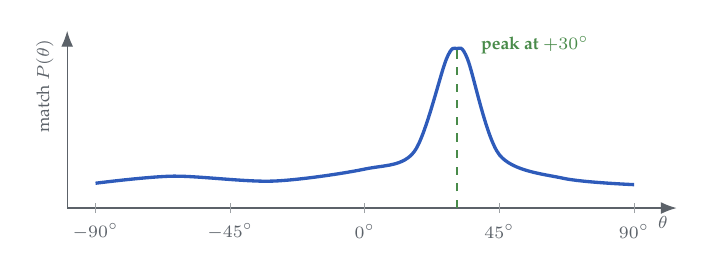
\begin{tikzpicture}[scale=0.9,transform shape]
    \draw[-{Latex[length=2mm]},softgray] (0,0) -- (8.6,0)
      node[below left,font=\scriptsize]{$\theta$};
    \draw[-{Latex[length=2mm]},softgray] (0,0) -- (0,2.5)
      node[rotate=90,font=\scriptsize,anchor=south east,yshift=2pt]{match $P(\theta)$};
    \foreach \t/\x in {-90/0.4, -45/2.3, 0/4.2, 45/6.1, 90/8.0}{
      \draw[softgray!60] (\x,-0.07) -- (\x,0.07);
      \node[font=\scriptsize,text=softgray] at (\x,-0.33) {$\t^\circ$};}
    \draw[ranblue,very thick] plot[smooth] coordinates
      {(0.4,0.35) (1.5,0.45) (2.9,0.38) (4.2,0.55) (4.9,0.8) (5.35,2.1)
       (5.5,2.25) (5.65,2.1) (6.1,0.75) (7.0,0.42) (8.0,0.33)};
    \draw[softgreen,dashed,thick] (5.5,0) -- (5.5,2.25);
    \node[font=\scriptsize\bfseries,text=softgreen] at (6.6,2.3)
      {peak at $+30^\circ$};
  \end{tikzpicture}

  \vspace{0.45em}
  \takeaway{This is a phased-array sweep with no moving parts:\\
    the beam is a \texttt{for}-loop over $\theta$, run \emph{after} reception.}

  \source{https://www.usenix.org/conference/nsdi13/technical-sessions/presentation/xiong}{Xiong and Jamieson, ArrayTrack, NSDI 2013}
\end{frame}

% Teaching note (180 s): break the clean picture. The wall echo is a real arrival
% with its own slope, so the spectrum honestly reports two directions. The question
% "which peak is the phone?" has NO answer on this axis -- leave it hanging; it is
% the cliffhanger that justifies the ToF section and SpotFi.
\begin{frame}{Multipath grows extra peaks}
  \vspace{0.2em}
  \centering
  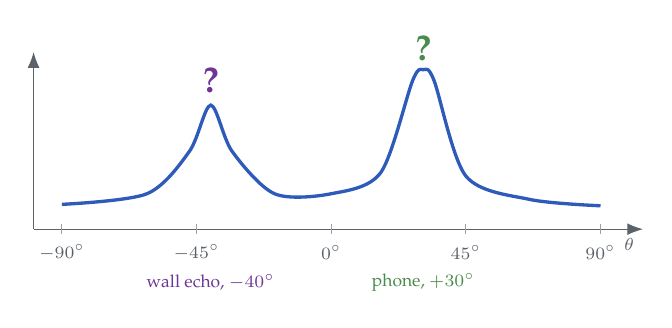
\begin{tikzpicture}[scale=0.9,transform shape]
    \draw[-{Latex[length=2mm]},softgray] (0,0) -- (8.6,0)
      node[below left,font=\scriptsize]{$\theta$};
    \draw[-{Latex[length=2mm]},softgray] (0,0) -- (0,2.5);
    \foreach \t/\x in {-90/0.4, -45/2.3, 0/4.2, 45/6.1, 90/8.0}{
      \draw[softgray!60] (\x,-0.07) -- (\x,0.07);
      \node[font=\scriptsize,text=softgray] at (\x,-0.33) {$\t^\circ$};}
    \draw[ranblue,very thick] plot[smooth] coordinates
      {(0.4,0.35) (1.6,0.5) (2.2,1.1) (2.5,1.75) (2.8,1.1) (3.4,0.5)
       (4.2,0.5) (4.9,0.8) (5.35,2.1) (5.5,2.25) (5.65,2.1) (6.1,0.75)
       (7.0,0.42) (8.0,0.33)};
    \node[font=\Large\bfseries,text=ranpurple] at (2.5,2.1) {?};
    \node[font=\Large\bfseries,text=softgreen] at (5.5,2.55) {?};
    \node[font=\scriptsize,text=ranpurple] at (2.5,-0.75) {wall echo, $-40^\circ$};
    \node[font=\scriptsize,text=softgreen] at (5.5,-0.75) {phone, $+30^\circ$};
  \end{tikzpicture}

  \vspace{0.4em}
  {\small
   \begin{itemize}\itemsep3pt
     \item Every arrival is real: the echo has its own slope, its own peak.
     \item On this axis alone, \textbf{nothing says which peak is the phone}.
     \item ArrayTrack's brute-force help: more antennas $\to$ sharper peaks
       (16 antennas $\to$ 23 cm median).
   \end{itemize}\par}

  \vspace{0.3em}
  \ask{We need a second ruler that tells the two peaks apart.\\
    Hold that thought --- first, let us sharpen this one.}
\end{frame}

% Teaching note (210 s): MUSIC without eigen-anxiety. The trick to say out loud:
% instead of asking "where IS signal?", ask "which directions are provably EMPTY?",
% then plot 1/emptiness. Hands-on versions: Princeton lab, Tsinghua tutorial code.
\begin{frame}{MUSIC, in one slide}
  \vspace{0.3em}
  {\small
   \begin{itemize}\itemsep4pt
     \item Collect many packets $\to$ average $\to$ a covariance of the antenna
       readings.
     \item Its eigenvectors split cleanly: a few span the \textbf{signal}
       (one per path), the rest span pure \textbf{noise}.
     \item A true arrival angle's steering vector is \emph{orthogonal} to the
       noise part.
     \item So plot $1/(\text{projection onto noise})$: division by almost-zero
       $\to$ needle-sharp spikes.
   \end{itemize}\par}

  \vspace{0.3em}
  \centering
  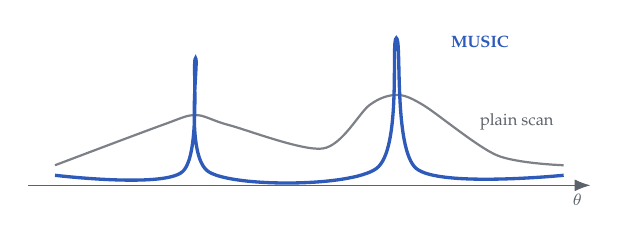
\begin{tikzpicture}[scale=0.85,transform shape]
    \draw[-{Latex[length=2mm]},softgray] (0,0) -- (8.4,0)
      node[below left,font=\scriptsize]{$\theta$};
    \draw[softgray!80,thick] plot[smooth] coordinates
      {(0.4,0.3) (2.0,0.9) (2.5,1.05) (3.0,0.9) (4.4,0.55) (5.1,1.2)
       (5.5,1.35) (5.9,1.2) (7.0,0.45) (8.0,0.3)};
    \draw[ranblue,very thick] plot[smooth] coordinates
      {(0.4,0.15) (2.3,0.2) (2.5,1.9) (2.7,0.2) (5.2,0.25) (5.5,2.2)
       (5.8,0.25) (8.0,0.15)};
    \node[font=\scriptsize,text=softgray] at (7.3,0.95) {plain scan};
    \node[font=\scriptsize\bfseries,text=ranblue] at (6.75,2.15) {MUSIC};
  \end{tikzpicture}

  \source{https://www.cs.princeton.edu/courses/archive/spring18/cos463/labs/lab5_preview.html}{Schmidt, IEEE Trans.\ AP 1986 \quad$\cdot$\quad Have a try: Princeton COS463 MUSIC lab; Tsinghua tutorial \texttt{naive\_aoa}}
\end{frame}
       % ruler 1: read across the antennas -> angle
%!TEX root = ./main.tex

\section[Distance]{Ruler 2: Distance, Read Across the Subcarriers}

% SECTION TIMING: 40:00--57:00 (5 frames). Chronos's and the Tsinghua tutorial's
% story. The symmetry IS the pedagogy: same trick as the last section, with the
% roles of "position" and "frequency" swapped. Say the sentence "difference across
% a small step beats wrapping" in both sections, verbatim.

% Teaching note (150 s): open by physically rotating your hand 90 degrees over the
% CSI grid: we just read columns (antennas); now we read rows (subcarriers). Then
% kill the naive hope with the 87-turns number from the wrapping frame.
\begin{frame}{Same trick: rotate the ruler}
  \vspace{0.3em}
  {\small Fix one antenna. Walk along the \textcolor{coreorange}{\textbf{frequency
    axis}} instead:\par}
  \vspace{0.2em}
  \centering
  {\large $\varphi(f) \;=\; -\,2\pi f \tau$
   \quad{\small\textcolor{softgray}{($\tau$ = time of flight $= r/c$)}}\par}

  \vspace{0.6em}
  \raggedright
  {\small
   \begin{itemize}\itemsep4pt
     \item One frequency alone is hopeless: our 5 m path is
       \textbf{87 turns} deep in wraps.
     \item But two \emph{nearby} frequencies differ by only
       $\Delta\varphi = 2\pi\,\Delta f\,\tau$ --- a tiny, unwrapped step.
     \item Same sentence as last section: a \textbf{difference across a small
       step beats wrapping}.
   \end{itemize}\par}

  \vspace{0.5em}
  \qa{Where do we get many nearby frequencies, measured at the same instant?}
     {You have known the answer since Class 8: \textbf{OFDM}. Every Wi-Fi packet
      is 52+ equally spaced tones, each reporting its own phase.}
\end{frame}

% Teaching note (210 s): THE frame of the section. Phase vs frequency is a straight
% line whose slope is the delay. Work the running example: 312.5 kHz per step gives
% ~1.9 degrees per subcarrier, ~120 degrees across a 20 MHz packet -- small but
% plainly measurable. And the wrap-around distance for the STEP is 960 m: no house
% is that big, so the slope never wraps indoors.
\begin{frame}{Two tones make a slope}
  \vspace{0.2em}
  \centering
  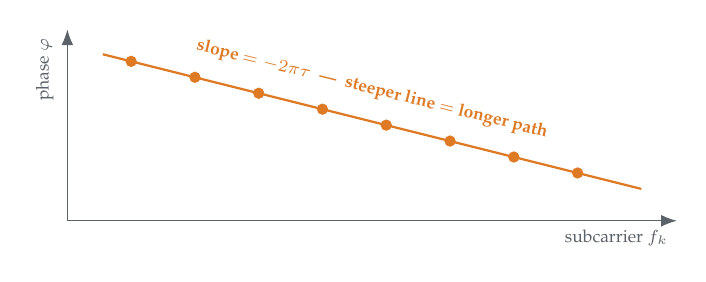
\begin{tikzpicture}[scale=0.9,transform shape]
    \draw[-{Latex[length=2mm]},softgray] (0,0) -- (8.6,0)
      node[below left,font=\scriptsize]{subcarrier $f_k$};
    \draw[-{Latex[length=2mm]},softgray] (0,0) -- (0,2.7)
      node[rotate=90,font=\scriptsize,anchor=south east,yshift=2pt]{phase $\varphi$};
    % measured points on a falling line
    \draw[coreorange,thick] (0.5,2.35) -- (8.1,0.45);
    \foreach \x in {0.9,1.8,2.7,3.6,4.5,5.4,6.3,7.2}{
      \pgfmathsetmacro{\y}{2.35-0.25*(\x-0.5)}
      \fill[coreorange] (\x,\y) circle (0.08);}
    \node[font=\scriptsize\bfseries,text=coreorange,rotate=-14] at (4.3,1.85)
      {slope $= -2\pi\tau$ \;---\; steeper line $=$ longer path};
  \end{tikzpicture}

  \vspace{0.35em}
  \begin{tcolorbox}[colback=green!5,colframe=softgreen,boxrule=0.7pt,arc=2pt,
    left=5pt,right=5pt,top=3pt,bottom=3pt,width=0.96\textwidth]
    \small\centering
    Running example, 5 m path: $1.9^\circ$ per 312.5 kHz subcarrier step,\\
    $\approx 120^\circ$ of total fall across one 20 MHz packet.
  \end{tcolorbox}

  \vspace{0.35em}
  {\small The step $\Delta f = 312.5$ kHz wraps only beyond
   $c/\Delta f = \textbf{960 m}$ --- indoors, never.\par}

  \source{https://www.usenix.org/conference/nsdi16/technical-sessions/presentation/vasisht}{Vasisht et al., Chronos, NSDI 2016 --- slides 11--31 walk exactly this argument}
\end{frame}

% Teaching note (180 s): multipath again, resolved the honest way: the measured
% line is a SUM of spirals, one per path, and the IFFT across subcarriers is the
% machine that sorts them by delay. Students know FFT from Class 8's OFDM frames;
% "the FFT's twin, run across the band" is enough.
\begin{frame}{The IFFT sorts the room by distance}
  \vspace{0.3em}
  \centering
  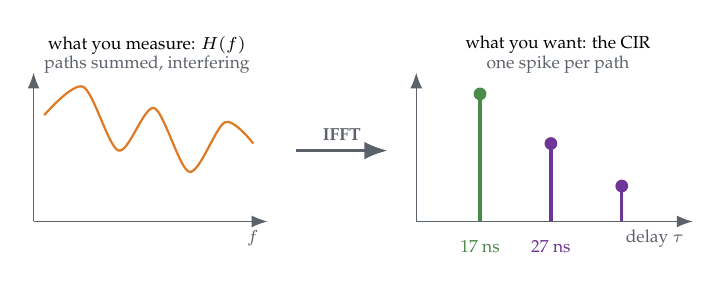
\begin{tikzpicture}[scale=0.9,transform shape]
    % CFR: a wiggly magnitude across frequency
    \draw[-{Latex[length=2mm]},softgray] (0,0) -- (3.3,0)
      node[below left,font=\scriptsize]{$f$};
    \draw[-{Latex[length=2mm]},softgray] (0,0) -- (0,2.1);
    \draw[coreorange,thick] plot[smooth] coordinates
      {(0.15,1.5) (0.7,1.9) (1.2,1.0) (1.7,1.6) (2.2,0.7) (2.7,1.4) (3.1,1.1)};
    \node[font=\scriptsize,align=center] at (1.6,2.35)
      {what you measure: $H(f)$\\{\scriptsize\color{softgray}paths summed,
        interfering}};
    % arrow
    \draw[-{Latex[length=3mm]},very thick,softgray] (3.7,1.0) -- (5.0,1.0)
      node[midway,above,font=\scriptsize\bfseries]{IFFT};
    % CIR: taps
    \draw[-{Latex[length=2mm]},softgray] (5.4,0) -- (9.3,0)
      node[below left,font=\scriptsize]{delay $\tau$};
    \draw[-{Latex[length=2mm]},softgray] (5.4,0) -- (5.4,2.1);
    \draw[softgreen,very thick] (6.3,0) -- (6.3,1.8);
    \fill[softgreen] (6.3,1.8) circle (0.09);
    \draw[ranpurple,very thick] (7.3,0) -- (7.3,1.1);
    \fill[ranpurple] (7.3,1.1) circle (0.09);
    \draw[ranpurple,very thick] (8.3,0) -- (8.3,0.5);
    \fill[ranpurple] (8.3,0.5) circle (0.09);
    \node[font=\scriptsize,text=softgreen] at (6.3,-0.35) {17 ns};
    \node[font=\scriptsize,text=ranpurple] at (7.3,-0.35) {27 ns};
    \node[font=\scriptsize,align=center] at (7.4,2.35)
      {what you want: the CIR\\{\scriptsize\color{softgray}one spike per path}};
  \end{tikzpicture}

  \vspace{0.5em}
  \takeaway{$H$ across frequency and the echoes across delay are a Fourier
    pair.\\The IFFT is the sorting machine.}

  \glossline{CFR = Channel Frequency Response ($H$ vs.\ $f$) \quad
    CIR = Channel Impulse Response ($H$ vs.\ $\tau$)}
\end{frame}

% Teaching note (210 s): the cold shower. Resolution = 1/bandwidth, period. Run the
% example: our two paths are 10 ns apart; a 20 MHz tap is 50 ns wide -- same tap,
% unresolvable. Let the table sink in before naming the two escapes.
\begin{frame}{Resolution is bandwidth}
  \vspace{0.3em}
  {\small Two CIR spikes merge unless their delays differ by
   $\gtrsim 1/B$:\par}

  \vspace{0.4em}
  \centering
  {\small
  \begin{tabular}{lccc}
    \toprule
    Channel width $B$ & tap width $1/B$ & in meters & our 5 m vs.\ 8 m paths? \\
    \midrule
    20 MHz  & 50 ns   & 15 m   & \textcolor{talkred}{merged} \\
    40 MHz  & 25 ns   & 7.5 m  & \textcolor{talkred}{merged} \\
    80 MHz  & 12.5 ns & 3.75 m & \textcolor{talkred}{barely} \\
    160 MHz & 6.25 ns & 1.9 m  & \textcolor{softgreen}{split} \\
    \bottomrule
  \end{tabular}\par}

  \vspace{0.6em}
  {\small Two escapes, and you have met both ideas today:\par}
  {\small
   \begin{itemize}\itemsep3pt
     \item \textbf{Super-resolution math} --- run MUSIC along the
       \textcolor{coreorange}{frequency axis} too (SpotFi, next section).
     \item \textbf{Buy bandwidth} --- hop across \emph{all} Wi-Fi bands and
       stitch the slopes into one giant sweep: Chronos, sub-nanosecond ToF.
   \end{itemize}\par}

  \source{https://www.usenix.org/conference/nsdi16/technical-sessions/presentation/vasisht}{Chronos stitches 2.4 and 5 GHz bands on commodity Wi-Fi cards}
\end{frame}

% Teaching note (210 s): the honesty frame; students who later touch real CSI will
% thank you. TX and RX clocks are strangers: absolute tau is biased by a different
% amount every packet. The rule that survives: trust differences, not absolutes --
% which is why this lecture only ever used slopes and steps.
\begin{frame}{What the clocks ruin}
  \vspace{0.3em}
  {\small\textbf{\textcolor{softgray}{Four lies in every raw CSI capture:}}\par}
  \vspace{0.3em}
  {\small
   \begin{itemize}\itemsep4pt
     \item \textbf{Unsynced clocks}: TX and RX never agree on $t = 0$;
       absolute $\tau$ is biased.
     \item \textbf{Packet detection delay}: the bias \emph{changes} packet to
       packet.
     \item \textbf{Carrier frequency offset}: a slow phase spin on top of
       everything.
     \item \textbf{Per-chain offsets}: each RF chain adds its own constant
       phase (calibrate once).
   \end{itemize}\par}

  \vspace{0.4em}
  {\small\textbf{\textcolor{softgreen}{What survives untouched:}} differences.
   Path-to-path delay gaps, the slope \emph{shape} across subcarriers,
   antenna-to-antenna steps.\par}

  \vspace{0.5em}
  \takeaway{Trust differences, not absolutes. (Chronos is, at heart,\\
    one long fight to win back the absolute.)}
\end{frame}
       % ruler 2: read across the subcarriers -> distance
%!TEX root = ./main.tex

\section[Both at once]{Both at Once: One Matrix, Two Rulers}

% SECTION TIMING: 57:00--66:00 (3 frames). SpotFi's move, on the running example.
% The payoff of the whole lecture: the matrix from the CSI section returns, now
% with both colored arrows on it, and the AoA cliffhanger ("which peak is the
% phone?") finally gets its answer -- the direct path is the SHORTEST one.

% Teaching note (150 s): bring back the exact grid students saw 40 minutes ago.
% Trace a column with a finger: angle. Trace a row: delay. Each path stamps the
% whole grid with one 2D twist -- so estimate (theta, tau) JOINTLY, per path.
\begin{frame}{The matrix returns}
  \vspace{0.4em}
  \centering
  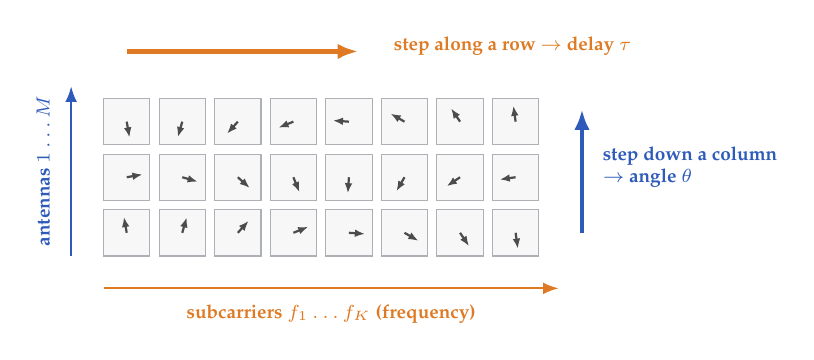
\begin{tikzpicture}[scale=0.98,transform shape]
    \csigrid
    \draw[-{Latex[length=2.6mm]},line width=1.6pt,ranblue]
      (6.2,0.3) -- (6.2,1.9);
    \node[font=\scriptsize\bfseries,text=ranblue,align=left] at (7.6,1.15)
      {step down a column\\$\to$ angle $\theta$};
    \draw[-{Latex[length=2.6mm]},line width=1.6pt,coreorange]
      (0.3,2.65) -- (3.3,2.65);
    \node[font=\scriptsize\bfseries,text=coreorange,align=left] at (5.3,2.72)
      {step along a row $\to$ delay $\tau$};
  \end{tikzpicture}

  \vspace{0.6em}
  {\small Each path twists the grid along \textbf{both} axes at once ---
   so fit both at once: treat every $(\text{antenna}, \text{subcarrier})$ cell
   as one sensor and run MUSIC over candidate \emph{pairs} $(\theta, \tau)$.\par}

  \vspace{0.4em}
  \takeaway{One measurement, two questions, answered jointly:\\
    2D MUSIC over $(\theta, \tau)$.}

  \source{https://dl.acm.org/doi/10.1145/2785956.2787487}{Kotaru et al., SpotFi, SIGCOMM 2015 --- Sec.\ 3: the 2D estimator and its smoothing trick}
\end{frame}

% Teaching note (180 s): the money picture. Two blobs, one per path, and the
% ambiguity from the AoA section dies: the wall echo sits at a LONGER delay, and
% light does not take shortcuts -- the direct path is always the earliest.
\begin{frame}{Every path is a peak in (angle, delay)}
  \vspace{0.3em}
  \centering
  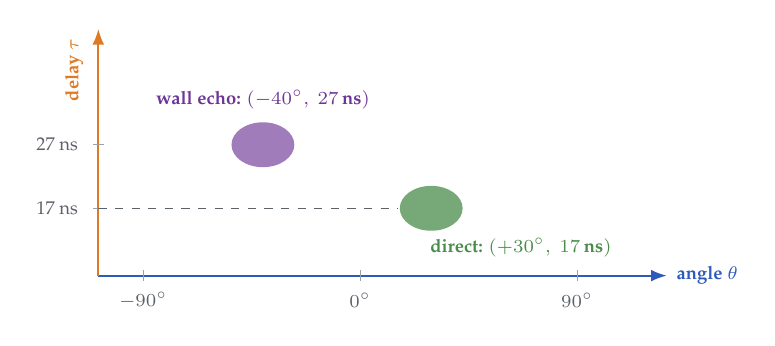
\begin{tikzpicture}[scale=0.95,transform shape]
    % axes
    \draw[-{Latex[length=2mm]},thick,ranblue] (0,0) -- (7.6,0)
      node[right,font=\scriptsize\bfseries,text=ranblue]{angle $\theta$};
    \draw[-{Latex[length=2mm]},thick,coreorange] (0,0) -- (0,3.3)
      node[rotate=90,font=\scriptsize\bfseries,text=coreorange,
           anchor=south east,yshift=2pt]{delay $\tau$};
    \foreach \t/\x in {-90/0.6, 0/3.5, 90/6.4}{
      \draw[softgray!60] (\x,-0.07) -- (\x,0.07);
      \node[font=\scriptsize,text=softgray] at (\x,-0.33) {$\t^\circ$};}
    \foreach \d/\y in {17/0.9, 27/1.75}{
      \draw[softgray!60] (-0.07,\y) -- (0.07,\y);
      \node[font=\scriptsize,text=softgray] at (-0.55,\y) {\d\ ns};}
    % the direct path blob
    \fill[softgreen,opacity=0.75] (4.45,0.9) ellipse (0.42 and 0.3);
    \node[font=\scriptsize\bfseries,text=softgreen] at (5.65,0.38)
      {direct: $(+30^\circ,\ 17\,\text{ns})$};
    % the wall echo blob
    \fill[ranpurple,opacity=0.65] (2.2,1.75) ellipse (0.42 and 0.3);
    \node[font=\scriptsize\bfseries,text=ranpurple] at (2.2,2.35)
      {wall echo: $(-40^\circ,\ 27\,\text{ns})$};
    % the rule
    \draw[softgray,dashed] (0,0.9) -- (4.0,0.9);
  \end{tikzpicture}

  \vspace{0.4em}
  \qa{Two peaks again --- which one is the phone \emph{now}?}
     {The \textbf{earliest} one. A reflection travels farther by definition, so
      the direct path has the smallest $\tau$. The delay axis breaks the tie the
      angle axis could not.}
\end{frame}

% Teaching note (150 s): land the result and close the loop to the hook card.
% SpotFi: 3 antennas, stock 802.11n AP, 40 cm median -- the number promised on
% slide one. One line on how several APs fuse bearings into a dot.
\begin{frame}{From (angle, delay) to a dot on the map}
  \vspace{0.3em}
  \centering
  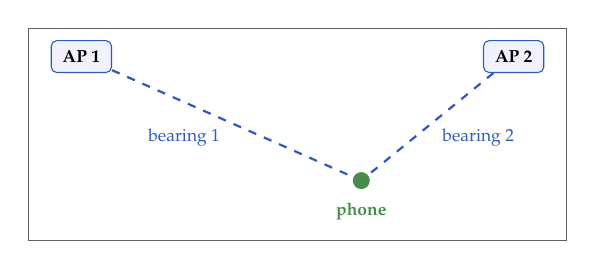
\begin{tikzpicture}[scale=0.9,transform shape]
    % floor plan
    \draw[softgray] (0,0) rectangle (7.6,3.0);
    % APs
    \node[draw=ranblue,fill=blue!5,rounded corners=2pt,minimum width=0.85cm,
          minimum height=0.45cm,font=\scriptsize\bfseries] (apa) at (0.75,2.6)
          {AP 1};
    \node[draw=ranblue,fill=blue!5,rounded corners=2pt,minimum width=0.85cm,
          minimum height=0.45cm,font=\scriptsize\bfseries] (apb) at (6.85,2.6)
          {AP 2};
    % bearings
    \draw[ranblue,thick,dashed] (apa) -- (4.7,0.85);
    \draw[ranblue,thick,dashed] (apb) -- (4.7,0.85);
    \fill[softgreen] (4.7,0.85) circle (0.12);
    \node[font=\scriptsize\bfseries,text=softgreen] at (4.7,0.42) {phone};
    \node[font=\scriptsize,text=ranblue] at (2.2,1.45) {bearing 1};
    \node[font=\scriptsize,text=ranblue] at (6.35,1.45) {bearing 2};
  \end{tikzpicture}

  \vspace{0.4em}
  {\small
   \begin{itemize}\itemsep3pt
     \item Each AP contributes its direct path's \textbf{bearing}; delays
       down-weight APs stuck behind reflections.
     \item Bearings intersect $\to$ a position --- no app, no extra hardware
       on the phone.
     \item SpotFi: stock 3-antenna 802.11n APs, \textbf{40 cm median error}.
   \end{itemize}\par}

  \vspace{0.35em}
  \takeaway{That is the hook card from slide one, cashed in.}
\end{frame}
    % both rulers on the same matrix -> one dot on the map
%!TEX root = ./main.tex

\section[Reality]{Reality Check}

% SECTION TIMING: 66:00--72:00 (2 frames). The honesty section the lecture earns
% its credibility with. Nothing new is taught here; every row points back at a
% frame that already explained it.

% Teaching note (180 s): read left column aloud in a textbook voice, right column
% in a lab voice. Every mismatch was covered earlier -- make them say WHERE.
\begin{frame}{The textbook vs.\ the hardware}
  \vspace{0.4em}
  \centering
  {\small\setlength{\tabcolsep}{5pt}
  \begin{tabular}{p{0.42\textwidth}p{0.45\textwidth}}
    \toprule
    \textbf{\textcolor{ranblue}{The textbook says}} &
    \textbf{\textcolor{talkred}{The hardware answers}} \\
    \midrule
    Phase encodes distance. &
    \ldots modulo 6 cm, 87 turns deep. \\[4pt]
    Subcarrier phases are clean. &
    A new detection delay tilts them every packet. \\[4pt]
    Antennas share one clock. &
    Each RF chain adds its own constant offset. \\[4pt]
    A CIR peak per path. &
    At 20 MHz, one tap is 15 m wide. \\[4pt]
    One target, standing still. &
    Chairs, doors, and people all reflect too. \\
    \bottomrule
  \end{tabular}\par}

  \vspace{0.7em}
  \takeaway{Every trick in this lecture was a \textbf{difference} ---\\
    slopes and steps survive what absolutes do not.}
\end{frame}

% Teaching note (180 s): three systems, three tricks, three honest numbers --
% each one is "the idea of one section of this lecture, pushed hard". Close with
% the standards line: the industry believed it enough to standardize it.
\begin{frame}{What real systems achieved}
  \vspace{0.3em}
  \centering
  {\small\setlength{\tabcolsep}{4.5pt}
  \begin{tabular}{llll}
    \toprule
    System & Pushes on & Hardware & Result \\
    \midrule
    ArrayTrack\ '13 & \textcolor{ranblue}{antenna axis} &
      16-antenna AP & 23 cm median \\[2pt]
    SpotFi\ '15 & \textcolor{ranblue}{both} \textcolor{coreorange}{axes},
      jointly & 3-antenna AP & 40 cm median \\[2pt]
    Chronos\ '16 & \textcolor{coreorange}{frequency axis} &
      one AP, band hops & sub-ns ToF \\
    \bottomrule
  \end{tabular}\par}

  \vspace{0.6em}
  {\small And the standards caught up:\par}
  {\small
   \begin{itemize}\itemsep3pt
     \item \textbf{802.11mc FTM}: round-trip ranging is in the Wi-Fi standard
       your phone ships with.
     \item \textbf{802.11bf}: a task group making \emph{sensing} itself a
       standard Wi-Fi feature.
   \end{itemize}\par}

  \source{https://www.ieee802.org/11/Reports/tgbf_update.htm}{ArrayTrack, NSDI'13 \;$\cdot$\; SpotFi, SIGCOMM'15 \;$\cdot$\; Chronos, NSDI'16 \;$\cdot$\; IEEE 802.11bf status}
\end{frame}
   % what the hardware ruins, and what systems still achieved
%!TEX root = ./main.tex

\section[Wrap-up]{Wrap-Up}

% SECTION TIMING: 72:00--75:00 (2 frames). Retrieval, then the bridge forward.

% Teaching note (120 s): retrieval practice. Cover the right column (overlay 1),
% ask the room to produce each ruler's axis and formula, then reveal.
\begin{frame}{One matrix, two axes, two rulers}
  \vspace{0.5em}
  \centering
  {\small\setlength{\tabcolsep}{4.5pt}
  \begin{tabular}{lll}
    \toprule
    Read $H[m,k]$\ldots & You get & Because \\
    \midrule
    \textcolor{ranblue}{down a column (antennas)} &
      \visible<2->{angle $\theta$} &
      \visible<2->{$\Delta\varphi = \frac{2\pi}{\lambda} d\sin\theta$} \\[4pt]
    \textcolor{coreorange}{along a row (subcarriers)} &
      \visible<2->{delay $\tau$ (distance)} &
      \visible<2->{$\Delta\varphi = 2\pi\,\Delta f\,\tau$} \\[4pt]
    \textcolor{softgreen}{both at once} &
      \visible<2->{$(\theta, \tau)$ peaks} &
      \visible<2->{2D MUSIC; earliest wins} \\
    \bottomrule
  \end{tabular}\par}

  \vspace{0.8em}
  \takeaway{Phase is a 6 cm ruler with no absolute markings.\\
    All of Wi-Fi sensing is reading its \textbf{differences} along the
    matrix's axes.}
\end{frame}

% Teaching note (60 s): the bridge. Class 13's papers run these exact two tricks
% on 5G uplink signals and on CSI biometrics; Class 14 reads the compressed CSI
% that beamforming feedback already broadcasts in the clear.
\begin{frame}{Where this goes next}
  \vspace{0.4em}
  {\small
   \begin{itemize}\itemsep5pt
     \item \textbf{Class 13 (practicum):} CARTS runs these tricks on 5G's own
       uplink reference signals; 2FiA reads breathing and heartbeat out of CSI.
     \item \textbf{Class 14:} the AP already \emph{broadcasts} compressed CSI
       --- 802.11 beamforming feedback --- and we will sense with that.
   \end{itemize}\par}

  \vspace{0.6em}
  {\small\textbf{Try it yourself} (both free, with code):\par}
  {\small
   \begin{itemize}\itemsep4pt
     \item Tsinghua \emph{Hands-on Wireless Sensing}:
       \blink{https://tns.thss.tsinghua.edu.cn/wst/docs/features}{CSI features
       tutorial} --- Matlab \texttt{naive\_aoa} / \texttt{naive\_tof}.
     \item Princeton COS463
       \blink{https://www.cs.princeton.edu/courses/archive/spring18/cos463/labs/lab5_preview.html}{MUSIC
       lab} --- build the AoA spectrum in NumPy.
   \end{itemize}\par}

  \vspace{0.7em}
  \ask{Your phone never opted in to any of this.\\
    Who should be allowed to run a ruler made of your Wi-Fi?}
\end{frame}


\end{document}
